\section{Examples Using \sysname}
\label{SEC:examples}

\cappos{This section is end-to-end examples that show all of the pieces coming
together.  Here, the paper discusses how to accomplish high level tasks
(key rotation, etc.) using the pieces from the prior section.}




\subsection{Introducing Docker Secrets Management}
\cappos{Taken from:
\url{https://blog.docker.com/2017/02/docker-secrets-management/}}

\cappos{This text needs to talk about how Notary, Swarmkit, Infrakit, etc.
work together to make this happen.}

We fundamentally believe that apps are safer if there is a standardized
interface for accessing secrets. Any good solution will also have to follow
security best practices, such as encrypting secrets while in transit;
encrypting secrets at rest; preventing secrets from unintentionally leaking
when consumed by the final application; and strictly adhere to the
principle of least-privilege, where an application only has access to the
secrets that it needs—no more, no less.

By integrating secrets into Docker orchestration, we are able to deliver a
solution for the secrets management problem that follows these exact
principles, as is shown in Figure~\ref{fig-swarm-arch}..

\begin{figure}[t]
  \center{}
  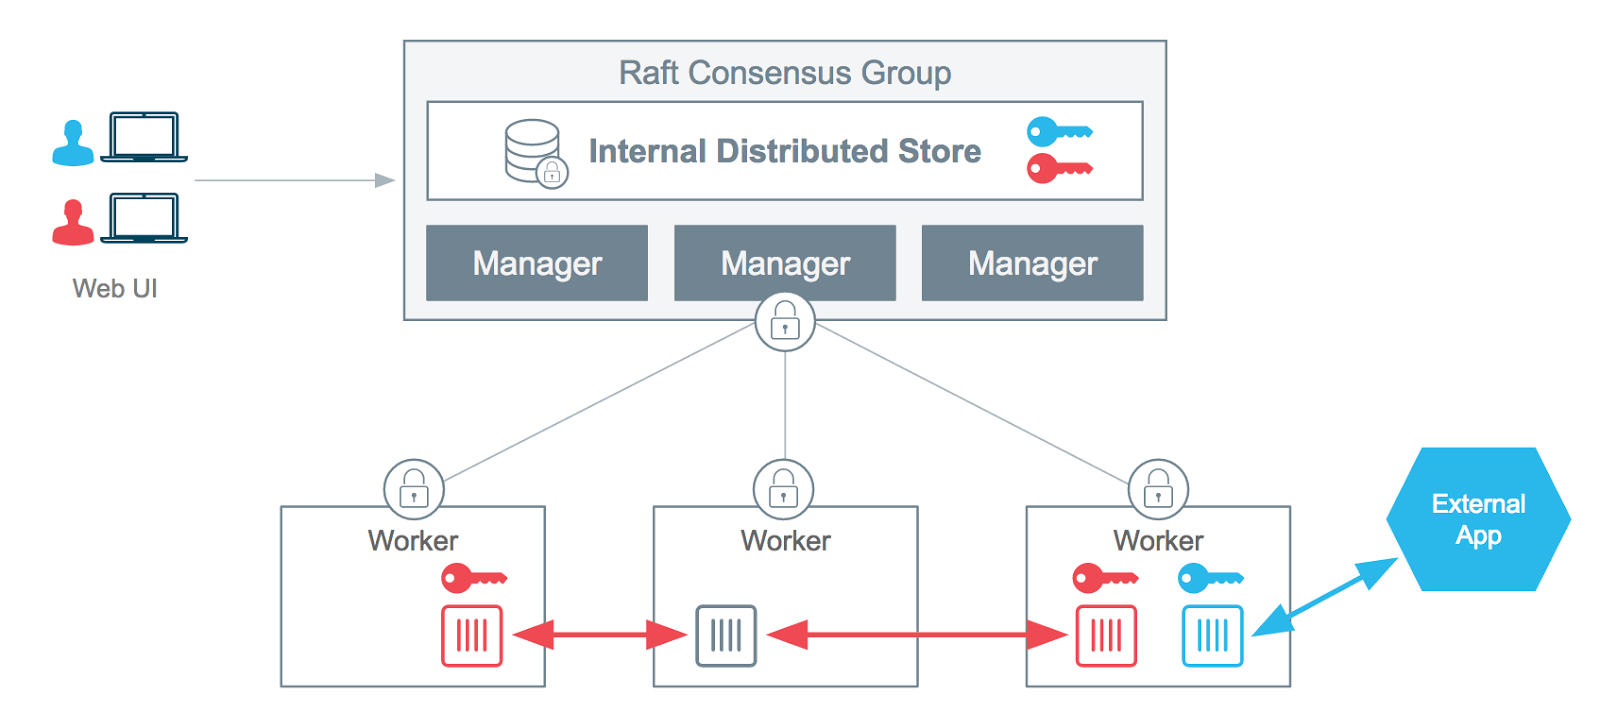
\includegraphics[width=.5\textwidth]{images/swarm_architecture.png}
  \caption{A high-level view of how the Docker swarm
mode architecture is applied to securely deliver a new type of object to
our containers: a secret object.
  \label{fig-swarm-arch} }
\end{figure}




In Docker, a secret is any blob of data, such as a password, SSH private
key, TLS Certificate, or any other piece of data that is sensitive in
nature. When you add a secret to the swarm (by running docker secret
create), Docker sends the secret over to the swarm manager over a mutually
authenticated TLS connection, making use of the built-in Certificate
Authority that gets automatically created when bootstrapping a new swarm.

 
\begin{quote}
\$ echo "This is a secret" | docker secret create my\_secret\_data -
\end{quote}
 

Once the secret reaches a manager node, it gets saved to the internal Raft
store, which uses NACL’s Salsa20Poly1305 with a 256-bit key to ensure no
data is ever written to disk unencrypted. Writing to the internal store
gives secrets the same high availability guarantees that the the rest of
the swarm management data gets.

When a swarm manager starts up, the encrypted Raft logs containing the
secrets is decrypted using a data encryption key that is unique per-node.
This key, and the node’s TLS credentials used to communicate with the rest
of the cluster, can be encrypted with a cluster-wide key encryption key,
called the unlock key, which is also propagated using Raft and will be
required on manager start.

When you grant a newly-created or running service access to a secret, one
of the manager nodes (only managers have access to all the stored secrets
stored) will send it over the already established TLS connection
exclusively to the nodes that will be running that specific service. This
means that nodes cannot request the secrets themselves, and will only gain
access to the secrets when provided to them by a manager – strictly for the
services that require them.

\begin{quote}
\$ docker service  create --name="redis" --secret="my\_secret\_data" redis:alpine
\end{quote}
 

The  unencrypted secret is mounted into the container in an in-memory
filesystem at /run/secrets/<secret\_name>.

\begin{quote}
\$ docker exec \$(docker ps --filter name=redis -q) ls -l /run/secrets
total 4
-r--r--r--    1 root     root            17 Dec 13 22:48 my\_secret\_data
\end{quote}
 

If a service gets deleted, or rescheduled somewhere else, the manager will
immediately notify all the nodes that no longer require access to that
secret to erase it from memory, and the node will no longer have any access
to that application secret.

\begin{quote}
\$ docker service update --secret-rm="my\_secret\_data" redis

\$ docker exec -it \$(docker ps --filter name=redis -q) cat /run/secrets/my\_secret\_data

cat: can't open '/run/secrets/my\_secret\_data': No such file or directory
\end{quote}


\bigskip
\cappos{This is pretty much similar text, but with different detail /
 emphasis.  Comes from:
\url{https://docs.docker.com/engine/swarm/secrets/\#about-secrets} }


In terms of Docker Swarm services, a secret is a blob of data, such as a
password, SSH private key, SSL certificate, or another piece of data that
should not be transmitted over a network or stored unencrypted in a
Dockerfile or in your application’s source code. In Docker 1.13 and higher,
you can use Docker secrets to centrally manage this data and securely
transmit it to only those containers that need access to it. Secrets are
encrypted during transit and at rest in a Docker swarm. A given secret is
only accessible to those services which have been granted explicit access
to it, and only while those service tasks are running.

You can use secrets to manage any sensitive data which a container needs at
runtime but you don’t want to store in the image or in source control, such
as:

\begin{itemize}
\item Usernames and passwords
\item TLS certificates and keys
\item SSH keys
\item Other important data such as the name of a database or internal server
\item Generic strings or binary content (up to 500 kb in size)
\end{itemize}

%Note: Docker secrets are only available to swarm services, not to
%standalone containers. To use this feature, consider adapting your
%container to run as a service with a scale of 1.

Another use case for using secrets is to provide a layer of abstraction
between the container and a set of credentials. Consider a scenario where
you have separate development, test, and production environments for your
application. Each of these environments can have different credentials,
stored in the development, test, and production swarms with the same secret
name. Your containers only need to know the name of the secret in order to
function in all three environments.

\subsubsection{How Docker manages secrets}
When you add a secret to the swarm, Docker sends the secret to the swarm
manager over a mutual TLS connection. The secret is stored in the Raft log,
which is encrypted. The entire Raft log is replicated across the other
managers, ensuring the same high availability guarantees for secrets as for
the rest of the swarm management data.

%Warning: Raft data is encrypted in Docker 1.13 and higher. If any of your
%Swarm managers run an earlier version, and one of those managers becomes
%the manager of the swarm, the secrets will be stored unencrypted in that
%node’s Raft logs. Before adding any secrets, update all of your manager
%nodes to Docker 1.13 to prevent secrets from being written to plain-text
%Raft logs.
When you grant a newly-created or running service access to a secret, the
decrypted secret is mounted into the container in an in-memory filesystem
at /run/secrets/<secret\_name>. You can update a service to grant it access
to additional secrets or revoke its access to a given secret at any time.

A node only has access to (encrypted) secrets if the node is a swarm
manager or if it is running service tasks which have been granted access to
the secret. When a container task stops running, the decrypted secrets
shared to it are unmounted from the in-memory filesystem for that container
and flushed from the node’s memory.

If a node loses connectivity to the swarm while it is running a task
container with access to a secret, the task container still has access to
its secrets, but cannot receive updates until the node reconnects to the
swarm.

You can add or inspect an individual secret at any time, or list all
secrets. You cannot remove a secret that a running service is using. See
Rotate a secret for a way to remove a secret without disrupting running
services.

In order to update or roll back secrets more easily, consider adding a
version number or date to the secret name. This is made easier by the
ability to control the mount point of the secret within a given container.

\subsubsection{Detailed example using secrets}

\cappos{Consider making an example that has enough interesting detail that
the reader gets all of the value from the three examples on:
\url{https://docs.docker.com/engine/swarm/secrets/\#examples}   This example
should be slightly more high level than it is currently.  It's too much of
a 'type this with me' guide and doesn't explain why or what is happening
enough..}

This simple example shows how secrets work in just a few commands. 
\begin{enumerate}
\item To add a secret to Docker, the user runs the {\tt docker 
secret create} command, as follows.   
\begin{quote}
\$ echo "This is a secret" | docker secret create my\_secret\_data -
\end{quote}

In this example, the command reads standard input because the last argument, 
which represents the file to read the secret from, is set to -.
\cappos{what's the point of this?  The secret ends up in your shell's
history this way?}


\item
Create a redis service and grant it access to the secret. By default, the
container can access the secret at /run/secrets/<secret\_name>, but you can
customize the file name on the container using the target option.

\begin{quote}
\$ docker service  create --name="redis" --secret="my\_secret\_data"
redis:alpine
\end{quote}

\item
Verify that the task is running without issues using docker service ps. If
everything is working, the output looks similar to this:

\begin{quote}
\$ docker service ps redis

ID            NAME     IMAGE         NODE              DESIRED STATE
CURRENT STATE          ERROR  PORTS
bkna6bpn8r1a  redis.1  redis:alpine  ip-172-31-46-109  Running
Running 8 seconds ago  
\end{quote}

If there were an error, and the task were failing and repeatedly
restarting, you would see something like this:

\begin{quote}
\$ docker service ps redis

NAME                      IMAGE         NODE  DESIRED STATE  CURRENT STATE
ERROR                      PORTS
redis.1.siftice35gla      redis:alpine  moby  Running        Running 4
seconds ago                             
 \_ redis.1.whum5b7gu13e  redis:alpine  moby  Shutdown       Failed 20
seconds ago      "task: non-zero exit (1)"  
 \_ redis.1.2s6yorvd9zow  redis:alpine  moby  Shutdown       Failed 56
seconds ago      "task: non-zero exit (1)"  
 \_ redis.1.ulfzrcyaf6pg  redis:alpine  moby  Shutdown       Failed about a
minute ago  "task: non-zero exit (1)"  
 \_ redis.1.wrny5v4xyps6  redis:alpine  moby  Shutdown       Failed 2
minutes ago       "task: non-zero exit (1)"
\end{quote}

\item
Get the ID of the redis service task container using docker ps , so that
you can use docker exec to connect to the container and read the contents
of the secret data file, which defaults to being readable by all and has
the same name as the name of the secret. The first command below
illustrates how to find the container ID, and the second and third commands
use shell completion to do this automatically.

\begin{quote}
\$ docker ps --filter name=redis -q

5cb1c2348a59

\$ docker exec \$(docker ps --filter name=redis -q) ls -l /run/secrets

total 4
-r--r--r--    1 root     root            17 Dec 13 22:48 my\_secret\_data

\$ docker exec \$(docker ps --filter name=redis -q) cat
/run/secrets/my\_secret\_data

This is a secret
\end{quote}

\item
Verify that the secret is not available if you commit the container.

\begin{quote}
\$ docker commit \$(docker ps --filter name=redis -q) committed\_redis

\$ docker run --rm -it committed\_redis cat /run/secrets/my\_secret\_data

cat: can't open '/run/secrets/my\_secret\_data': No such file or directory
\end{quote}

\item
Try removing the secret. The removal fails because the redis is running and
has access to the secret.

\begin{quote}
\$ docker secret ls

ID                          NAME                CREATED             UPDATED
wwwrxza8sxy025bas86593fqs   my\_secret\_data      4 hours ago         4 hours
ago


\$ docker secret rm my\_secret\_data

Error response from daemon: rpc error: code = 3 desc = secret
'my\_secret\_data' is in use by the following service: redis
\end{quote}

\item
Remove access to the secret from the running redis service by updating the
service.

\begin{quote}
\$ docker service update --secret-rm="my\_secret\_data" redis
\end{quote}

\item
Repeat steps 3 and 4 again, verifying that the service no longer has access
to the secret. The container ID will be different, because the service
update command redeploys the service.

\begin{quote}
\$ docker exec -it \$(docker ps --filter name=redis -q) cat
/run/secrets/my\_secret\_data

cat: can't open '/run/secrets/my\_secret\_data': No such file or directory
\end{quote}

\item
Stop and remove the service, and remove the secret from Docker.

\begin{quote}
\$ docker service rm redis

\$ docker secret rm my\_secret\_data
\end{quote}

\end{enumerate}




\subsection{How PKI works in swarm mode}

\cappos{taken from:
\url{https://docs.docker.com/engine/swarm/how-swarm-mode-works/pki/}}


The swarm mode public key infrastructure (PKI) system built into Docker
Engine makes it simple to securely deploy a container orchestration system.
The nodes in a swarm use mutual Transport Layer Security (TLS) v1.2 or
greater to authenticate, authorize, and encrypt the communications between 
themselves and other nodes in the swarm.

When you create a swarm by running docker swarm init, the Docker Engine
designates itself as a manager node. By default, the manager node generates
itself a new root Certificate Authority (CA) along with a key pair to
secure communications with other nodes that join the swarm. If you prefer,
you can pass the --external-ca flag to specify a root CA external to the
swarm. Refer to the docker swarm init CLI reference.

The manager node also generates two tokens to use when you join additional
nodes to the swarm: one worker token and one manager token. Each token
includes the digest of the root CA’s certificate and a randomly generated
secret. When a node joins the swarm, it uses the digest to validate the
root CA certificate from the remote manager. It uses the secret to ensure
the node is an approved node.

Each time a new node joins the swarm, the manager issues a certificate to
the node that contains a randomly generated node id to identify the node
under the certificate common name (CN) and the role under the
organizational unit (OU). The node id serves as the cryptographically
secure node identity for the lifetime of the node in the current swarm.


For example, Figure~\ref{fig-swarm-pki} shows ... \cappos{Walk us through 
some interesting actions with the worker nodes, etc.  The existing figure
is nice, but it should show some interesting action (such as node join), 
instead of only showing the resulting steady state...  }

\begin{figure}[t]
  \center{}
  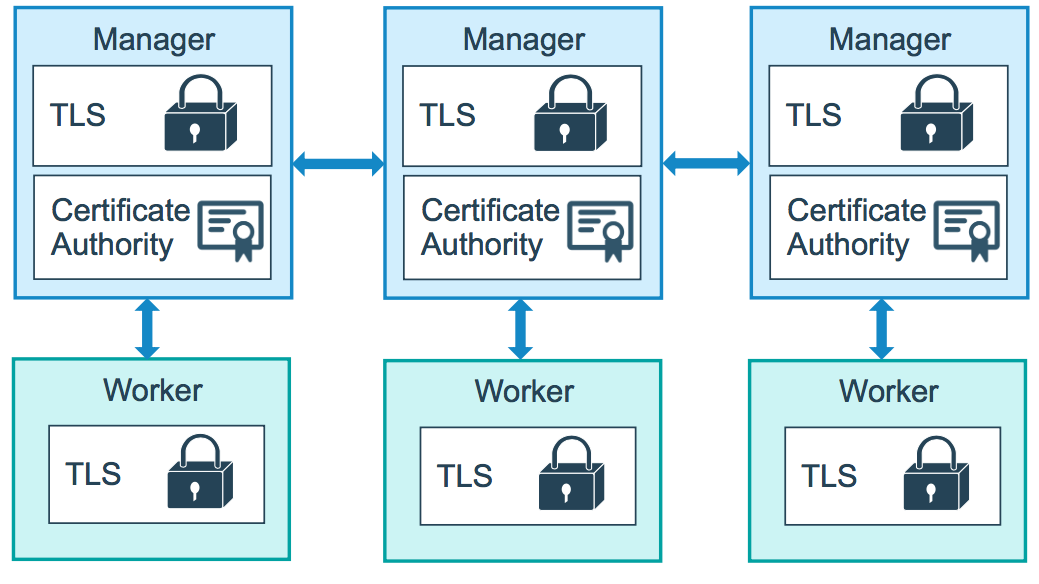
\includegraphics[width=.5\textwidth]{images/swarm-mode-pki.png}
  \caption{This figure illustrates how worker manager nodes and worker nodes 
encrypt communications using TLS
  \label{fig-swarm-pki} }
\end{figure}

The example below shows the information from a certificate from a worker
node:

\begin{quote}
Certificate:
    Data:
        Version: 3 (0x2)
        Serial Number:
            3b:1c:06:91:73:fb:16:ff:69:c3:f7:a2:fe:96:c1:73:e2:80:97:3b
        Signature Algorithm: ecdsa-with-SHA256
        Issuer: CN=swarm-ca
        Validity
            Not Before: Aug 30 02:39:00 2016 GMT
            Not After : Nov 28 03:39:00 2016 GMT
        Subject: O=ec2adilxf4ngv7ev8fwsi61i7, OU=swarm-worker,
CN=dw02poa4vqvzxi5c10gm4pq2g
...snip...
\end{quote}

By default, each node in the swarm renews its certificate every three
months. You can run docker swarm update --cert-expiry <TIME PERIOD> to
configure the frequency for nodes to renew their certificates. The minimum
rotation value is 1 hour. Refer to the docker swarm update CLI reference.


 



...



